\documentclass[12pt]{article}

\usepackage[utf8x]{inputenc}
\usepackage[T1]{fontenc}
\usepackage[english]{babel}

\usepackage{amsmath,amssymb,siunitx,tikz,listings}
\usetikzlibrary{calc,intersections}

\lstset{texcl,basicstyle=\footnotesize,frame=single,stringstyle=\ttfamily,language=tex,tabsize=4,backgroundcolor=\color{green!50!blue!20!white}}

\usepackage{hyperref}
\usepackage{float}
\floatstyle{boxed}
\restylefloat{figure}

\hypersetup{
	colorlinks,
	linkcolor={black!90!red},
	citecolor={black!90!blue},
	urlcolor={black!90!green}
}

\begin{document}
\section{Geometry of an equaliteral triangle}\label{geometrieabschnitt}
\begin{figure}[H]
\centering
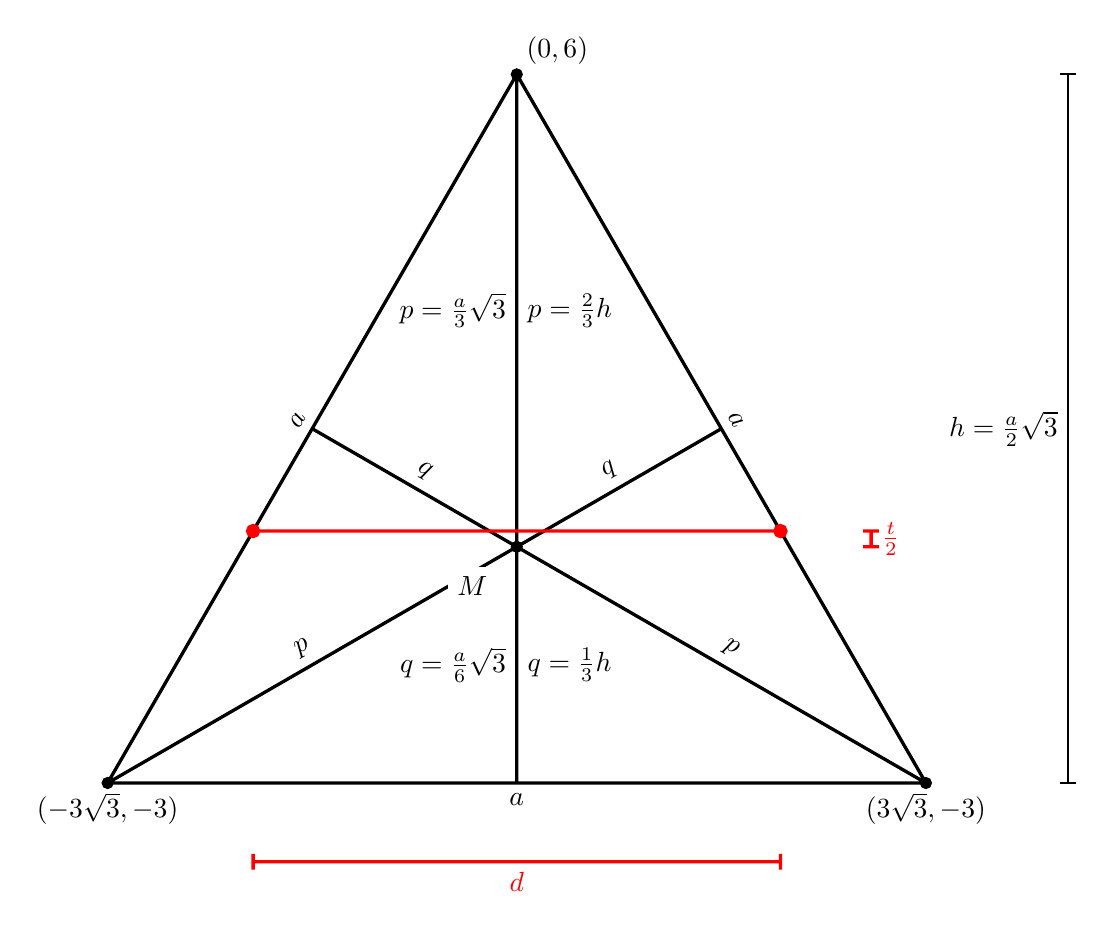
\begin{tikzpicture}[
	scale=1,
	auto,
	every node/.style={transform shape}
]
%\draw[step=0.1cm,black!5!white] (-9,-9)grid(9,9);
%\draw[step=0.5cm,black!20!white] (-9,-9)grid(9,9);
%\draw[step=1cm,black!50!white] (-9,-9)grid(9,9);
%\node[below left,draw=none] at (-9,-9){$-9$};
%\foreach \x in {-8,...,9}{
%	\node[left=0.29cm,draw=none] at (-9,\x){$\x$};
%	\node[below=0.27cm,draw=none] at (\x,-9){$\x$};
%}
\draw[very thick] (0,6)coordinate(e1) to node[sloped]{$a$} ({3*sqrt(3)},-3)coordinate(e2) to node[sloped,swap]{$a$} ({-3*sqrt(3)},-3)coordinate(e3) to node[sloped]{$a$} cycle to node{$p=\frac{2}{3}h$}node[swap]{$p=\frac{a}{3}\sqrt{3}$} (0,0)coordinate(m) to node{$q=\frac{1}{3}h$}node[swap]{$q=\frac{a}{6}\sqrt{3}$} (0,-3)(e2) to node[sloped]{$p$} (m) to node[sloped]{$q$} ($(m)!-0.5!(e2)$)(e3) to node[sloped]{$p$} (m) to node[sloped]{$q$}($(m)!-0.5!(e3)$);
\draw[fill=black] let \p1=(e1) in (\p1)circle(2pt)node[above right,draw=none,fill=none]{$(0,6)$};
\draw[fill=black] let \p1=(e2) in (\p1)circle(2pt)node[below,draw=none,fill=none]{$(3\sqrt{3},-3)$};
\draw[fill=black] let \p1=(e3) in (\p1)circle(2pt)node[below,draw=none,fill=none]{$(-3\sqrt{3},-3)$};
\draw[fill=black] let \p1=(m) in (\p1)circle(2pt)node[below left=0.25cm,fill=white]{$M$};
\draw[thick] (6.9,-3)--++(0.2,0)++(-0.1,0)--++(0,9)node[midway,left]{$h=\frac{a}{2}\sqrt{3}$}--++(-0.1,0)--++(0.2,0);
\path[name path=p1] (e3) to (e1) to (e2);
\path[name path=p2] let \p1=(e3),\p2=(e2) in (\x1,0.2) to (\x2,0.2);
\draw[very thick,name intersections={of=p1 and p2},red,fill=red] (intersection-1)circle(2pt)coordinate(i1) to (intersection-2)circle(2pt)coordinate(i2);
\draw[very thick,red] let \p1=(i1),\p2=(i2) in (\x1,-3.9)--++(0,-0.2)++(0,0.1) to node[swap,red]{$d$} (\x2,-4)++(0,-0.1)--++(0,0.2)(4.4,\y1)--++(0.2,0)++(-0.1,0) to node[red]{$\frac{t}{2}$} (4.5,0)++(-0.1,0)--++(0.2,0);
\end{tikzpicture}
\end{figure}
\begin{minipage}[l]{0.48\textwidth}
The node will be created with a textbox, whose dimensions will be expanding in x- and y-Dimension. The question we need to solve is: how do we need to choose $a$ if we have a textbox with width $d$ and height $t$ (Half of the textbox will be located \textit{under} the middle)?
\end{minipage}
\begin{minipage}[r]{0.48\textwidth}
\begin{figure}[H]
\centering
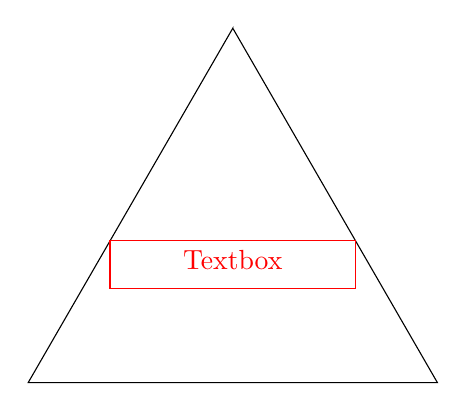
\begin{tikzpicture}[
	scale=0.75,
	auto
]
\draw[name path=p1] (0,4) to ({2*sqrt(3)},-2) to ({-2*sqrt(3)},-2) to cycle;
\path[name path=p2] ({2*sqrt(3)},0.4) to ({-2*sqrt(3)},0.4);
\draw[name intersections={of=p1 and p2},red] let \p1=(intersection-1),\p2=(intersection-2) in (\x1,-0.4)rectangle(\x2,0.4);
\path (intersection-1) to node[red]{Textbox} (intersection-2);
\end{tikzpicture}
\end{figure}
\end{minipage}\\\clearpage
\noindent We solve this by solving the following problem, and inverting it's answer afterwards:\\
Given the side $a$ of an equaliteral triangle and a displacement $\frac{t}{2}$ to its middlepoint, what is the distance $d$?\\
First: let's rename $\frac{t}{2}$ to $x$, and define a linear function $f(x)=n\cdot x + m$, which gives us the width of the triangle at displacement-height $x$.\\
$f$ fullfills obviously the following conditions:
\begin{equation}
f\left(-\frac{a}{6}\sqrt{3}\right)=a\label{ganzeseite}
\end{equation}
For a displacement of $-\frac{a}{6}\sqrt{3}$, $d$ lies exactly on the bottom triangle side, whose length is $a$.
\begin{equation}
f\left(\frac{a}{3}\sqrt{3}\right)=0\label{nullseite}
\end{equation}
For a displacement of $\frac{a}{3}\sqrt{3}$, $d$ lies exactly in the tip of the triangle, therefore its length needs to be $\num{0}$.
With \autoref{ganzeseite} and \autoref{nullseite} we get:
\begin{align}
&\begin{cases} n\cdot\left(-\frac{a}{6}\sqrt{3}\right)+m&=a\\ n\cdot\frac{a}{3}\sqrt{3}+m&=0\end{cases}\qquad (I)-(II)\nonumber\\
\Leftrightarrow &\begin{cases} -n\cdot\frac{a}{2}\sqrt{3}&=a\quad\Rightarrow\quad n=-\frac{2}{3}\sqrt{3}\\ n\cdot\frac{a}{3}\sqrt{3}+m&=0\quad\Rightarrow\quad -\frac{2}{3}\sqrt{3}\cdot\frac{a}{3}\sqrt{3}+m=0\quad\Rightarrow\quad m=\frac{2}{3}a\end{cases}\label{geloestefunktion}
\end{align}
With \autoref{geloestefunktion} we get $f(x)=-\frac{2}{3}\sqrt{3}\cdot x+\frac{2}{3}a$. For $d$, we find then the condition, by re-replacing $x$ with $\frac{t}{2}$ again, $d=f\left(\frac{t}{2}\right)$:
\begin{align}
d&=f\left(\frac{t}{2}\right)\nonumber\\
\Leftrightarrow d&=\frac{2}{3}\left(a-\sqrt{3}\cdot\frac{t}{2}\right)\nonumber\\
\Leftrightarrow a&=\frac{3}{2}d+\frac{t}{2}\sqrt{3}\label{geloesteseite}
\end{align}
More valuable than the length of the side is the coordinate of the top tip, which is then given by $p=\frac{a}{3}\sqrt{3}$ using \autoref{geloesteseite}. This leads us to the coordinate $(0,\frac{d}{2}\sqrt{3}+\frac{t}{2})$.
\section{Declaring the equaliteral triangle node shape in pgf}
A new shape is declared in pgf using
\begin{lstlisting}[mathescape]
\pgfdeclarenewshape{shapename}{shapecode}
\end{lstlisting}
\noindent \lstinline{shapename} will be "equaltri", since we are free with choosing it. \lstinline{shapecode} is the tricky part, since here we need to fix the pgf-layers on such way, that it will work in the end, so let's begin.\\
The first important point for \lstinline{shapecode} are saved anchors. This anchors are saved in the pdf along with every node, that has been drawn. Therefore, a shape should have as less as possible saved anchors, even though one should not forget, that it needs at least one of those in order to work properly. We start by defining a saved anchor. Since our triangle is equaliteral, there is only one degree of freedom. By choosing our saved anchor wisely, we shouldn't need more than one:\\
If we choose the center as saved anchor, math might get easy due to the symmetry. But sadly, the point $(0,0)$ does not store any information about textwidth and textheight (on which we only have access while saved anchors are created more to this point later on), which would force ous to create a second saved anchor somewhere else, for example in one of the triangle tips, or even better at a corner of the textbox. The other way around, choosing the textboxcorner as saved anchor is enough to reconstruct the whole triangle: since we compute the positions out of the texboxes size, remembering it's size will always be sufficient to reconstruct all coordinates inside the triangle using \autoref{geloestefunktion}.\\
We compute the saved anchor like given in \autoref{savedanchor}, and store the values in \lstinline{\pgf@x} and \lstinline{\pgf@y}, which is the pgf-method of returning points out of subroutines. With this restrictions, the command looks as follows:
\begin{lstlisting}[caption={The creation of one saved anchor called $\backslash$top},label=savedanchor]
\makeatletter
\pgfdeclareshape{equaltri}{
	\savedanchor{\text}{
		\pgfmathsetlength\pgf@x{-0.5\wd\pgfnodeparttextbox}
		\pgfmathsetlength\pgf@y{-0.5\ht\pgfnodeparttextbox}
	}
}
\makeatother
\end{lstlisting}
\lstinline{\makeatletter} and \lstinline{\makeatother} are required in order to have access to \lstinline{\pgf@x} and \lstinline{\pgf@y}. Make sure you use a tex-macro as name, which means something with a $\backslash$ at the beginning. But this is not sufficient yet, we specified a saved anchor which holds the the textbox-information on a smart way. We did not tell pgf where the text should be, and by trying to compile this (you need to draw a tikzpicture in your document, which draws at least one node of equaltri), you will get an error. Let's first handle that.\\
The error is thrown because pgf places a node accordingly to it's anchor called center. Obviously, that anchor is not specified yet. The difference between anchors and saved anchors is, that anchors will only be computet if they are requested, for example if you want do draw from \lstinline{(mynode.north west)} to somewhere, or pgf uses the center anchor to position the node, while saved anchors are computed and safed when the node is created. Therefore, only saved anchors should access the global variable \lstinline!\pgfnodeparttextbox! or similar ones, since a normal anchor will be called at times, when those variables don't hold the information about the required node anymore. All information the anchor can use, is the information which is stored in our saved anchor, in our case \lstinline{\text}. However, center will not need that information since it will only point to the origin of the shape, which can be accessed easily by \lstinline{\pgfpointorigin}, which translates to $(0,0)$, because inside \lstinline!\pgfdeclareshape{name}{command}! pgf-coordinates such as \lstinline!\pgfpointorigin! or \lstinline!\pgfpoint{x}{y}! are interpreted as relative coordinates to it's origin.\\
Let's create now the needed anchors (the shown code must be placed immediately under the \lstinline|\savedanchor|-part, still inside \lstinline!\pgfdeclareshape{}{}!)
\begin{lstlisting}[caption=Creation of the one (two) necessary anchor(s),label=necessesaryanchors]
\anchor{center}{
	\pgfpointorigin
}
\anchor{text}{
	\text
}
\end{lstlisting}
Note, that \lstinline$\pgf@x=<some number>$ works perfectly, while\\\lstinline$\pgf@x=<some computation>$ does not. TeX can only compute mathematical expressions, if they're given in a \lstinline!\pgfmathset<type>{name}{expression}! manner. Since \lstinline!\pgf@x! and \lstinline!\pgf@y! are lengths, \lstinline!<type>! needs to be length in our case (see \autoref{savedanchor}).\\
\def\k{0.45}
\begin{minipage}[l]{\k\textwidth}
The really needed anchor in our case is center. TeX uses center to position the node at a given or self-chosen coordinate.\\
If the text of your node is not empty, TeX will use the anchor text in addition to place the textbox inside the node. Be aware, that the point specified by text will be the lower left corner of the textbox, not the middle, therefore we shift text by half the dimensions of it's box (already done in the saved anchor), which should be aligned in the middle of our triangle.
\end{minipage}
\begin{minipage}[r]{\k\textwidth}
\begin{figure}[H]
\begin{center}
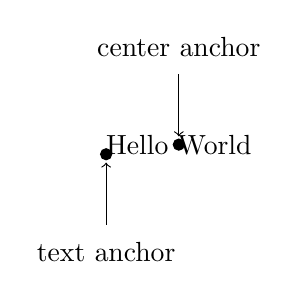
\begin{tikzpicture}
\makeatletter
\pgfdeclareshape{equaltri}{
	\savedanchor{\text}{
		\pgfmathsetlength\pgf@x{-0.5\wd\pgfnodeparttextbox}
		\pgfmathsetlength\pgf@y{-0.5\ht\pgfnodeparttextbox}
	}
	\anchor{top}{
		\text
		\pgfmathsetlength\pgf@y{-sqrt(3)*\pgf@x+sqrt(3)*0.5mm-\pgf@y+0.25mm}
		\pgfmathsetlength\pgf@x{0}
	}
	\anchor{center}{
		\pgfpointorigin
	}
	\anchor{text}{
		\text
	}
}
\makeatother
\node[equaltri](n){Hello World};
\draw[fill=black] (n.center)circle(2pt)node[above=1cm](ca){center anchor}(n.text)circle(2pt)node[below=1cm](ta){text anchor}(n.center)edge[<-, shorten <= 3pt, shorten >= 3pt](ca)(n.text)edge[<-, shorten <= 3pt, shorten >= 3pt](ta);
\end{tikzpicture}
\end{center}\caption{The two defined anchors.}
\end{figure}
\end{minipage}\\
By calling \lstinline!\text!, \lstinline!\pgf@x! and \lstinline!\pgf@y! will be set to the values saved in \lstinline!\text!. One may now ask why we need to create an anchor if we have already a saved anchor. The problem is, that TikZ from the outside of the shape has no access to saved anchors. We need the parsing anchor text to enable access from outside.\\
Compiling now, we see that there won't be any errors, as long as you copied everything correctly. If you get still errors, compare your code with \autoref{elementaresbeispiel}.\\
To draw the shape, TikZ need to know that it should do it, so let's pass \lstinline!draw! to our node: \lstinline!\node[equaltri,draw]{Hello World}!. Well the result is\ldots{} not really impressive. The reason is, that we didn't specify any drawing work yet. In fact, pgf does not even have any chance to know, that we want a triangle, we didn't specify it yet.\\
\begin{minipage}[l]{\k\textwidth}
For this task, we have two possibilities: either the \lstinline!\backgroundpath{}!- or the \lstinline!\foregroundpath{}!-command. As you might already have figured out by yourself, the \lstinline!\backgroundpath! will be drawn behind the text, \lstinline!\foregroundpath! in front of the text. Both paths can be used for something, but keep in mind, that the fill operation in combination with a triangle in \lstinline!\foregroundpath! will hide the text with the fill color. Therefore we should stick to \lstinline!\backgroundpath! for surrounding shapes:
\end{minipage}
\begin{minipage}[r]{\k\textwidth}
\begin{figure}[H]
\begin{center}
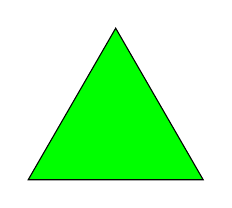
\begin{tikzpicture}[scale=0.7]
\makeatletter
\pgfdeclareshape{equaltri2}{
	\savedanchor{\text}{
		\pgfmathsetlength\pgf@x{-0.5\wd\pgfnodeparttextbox}
		\pgfmathsetlength\pgf@y{-0.5\ht\pgfnodeparttextbox}
	}
	\anchor{top}{
		\text
		\pgfmathsetlength\pgf@y{-sqrt(3)*\pgf@x+sqrt(3)*0.5mm-\pgf@y+0.25mm}
		\pgfmathsetlength\pgf@x{0}
	}
	\anchor{bottom left}{
		\text \pgf@xa=\pgf@x
		\pgfmathsetlength\pgf@x{-sqrt(3)/2*(-sqrt(3)*\pgf@xa+sqrt(3)*0.5mm-\pgf@y+0.25mm)}
		\pgfmathsetlength\pgf@y{-(-sqrt(3)*\pgf@xa+sqrt(3)*0.5mm-\pgf@y+0.25mm)/2}
	}
	\anchor{bottom right}{
		\text \pgf@xa=\pgf@x
		\pgfmathsetlength\pgf@x{-1.5*\pgf@xa+0.75mm-sqrt(3)*\pgf@y/2+0.125mm}
		\pgfmathsetlength\pgf@y{sqrt(3)*\pgf@xa/2-sqrt(3)*0.25mm+\pgf@y/2-0.125mm}
	}
	\anchor{center}{
		\pgfpointorigin
	}
	\anchor{text}{
		\text
	}
	\foregroundpath{
		\text
		\pgfmathsetlength\pgf@ya{-sqrt(3)*\pgf@x+sqrt(3)*0.5mm-\pgf@y+0.25mm}
		\pgfmathsetlength\pgf@xa{0}
		\pgfpathmoveto{\pgfpoint{\pgf@xa}{\pgf@ya}}
		\pgfmathsetlength\pgf@xa{-sqrt(3)*\pgf@ya/2}
		\pgfmathsetlength\pgf@ya{-\pgf@ya/2}
		\pgfpathlineto{\pgfpoint{\pgf@xa}{\pgf@ya}}
		\pgfmathsetlength\pgf@xa{-\pgf@xa}
		\pgfpathlineto{\pgfpoint{\pgf@xa}{\pgf@ya}}
		\pgfpathclose
	}
}
\makeatother
\node[equaltri2,draw,fill=green,transform shape](n){Hello World};
\end{tikzpicture}\\
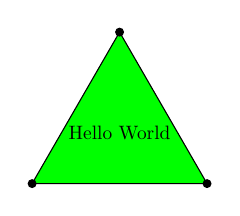
\begin{tikzpicture}[scale=0.7]
\makeatletter
\pgfdeclareshape{equaltri}{
	\savedanchor{\text}{
		\pgfmathsetlength\pgf@x{-0.5\wd\pgfnodeparttextbox}
		\pgfmathsetlength\pgf@y{-0.5\ht\pgfnodeparttextbox}
	}
	\anchor{top}{
		\text
		\pgfmathsetlength\pgf@y{-sqrt(3)*\pgf@x+sqrt(3)*0.5mm-\pgf@y+0.25mm}
		\pgfmathsetlength\pgf@x{0}
	}
	\anchor{bottom left}{
		\text \pgf@xa=\pgf@x
		\pgfmathsetlength\pgf@x{1.5*\pgf@xa-0.75mm+sqrt(3)*\pgf@y/2-sqrt(3)*0.125mm}
		\pgfmathsetlength\pgf@y{sqrt(3)*\pgf@xa/2-sqrt(3)*0.25mm+\pgf@y/2-0.125mm}
	}
	\anchor{bottom right}{
		\text \pgf@xa=\pgf@x
		\pgfmathsetlength\pgf@x{-1.5*\pgf@xa+0.75mm-sqrt(3)*\pgf@y/2+sqrt(3)*0.125mm}
		\pgfmathsetlength\pgf@y{sqrt(3)*\pgf@xa/2-sqrt(3)*0.25mm+\pgf@y/2-0.125mm}
	}
	\anchor{center}{
		\pgfpointorigin
	}
	\anchor{text}{
		\text
	}
	\anchor{north west}{
		\text
		\pgfmathsetlength\pgf@y{-sqrt(3)*\pgf@x+sqrt(3)*0.5mm-\pgf@y+0.25mm}
		\pgfmathsetlength\pgf@x{-sqrt(3)*\pgf@y/2}
	}
	\anchor{north}{
		\text
		\pgfmathsetlength\pgf@y{-sqrt(3)*\pgf@x+sqrt(3)*0.5mm-\pgf@y+0.25mm}
		\pgfmathsetlength\pgf@x{0}
	}
	\anchor{north east}{
		\text
		\pgfmathsetlength\pgf@y{-sqrt(3)*\pgf@x+sqrt(3)*0.5mm-\pgf@y+0.25mm}
		\pgfmathsetlength\pgf@x{sqrt(3)*\pgf@y/2}
	}
	\anchor{west}{
		\text
		\pgfmathsetlength\pgf@y{-sqrt(3)/4*\pgf@x+sqrt(3)*0.125mm-\pgf@y/4+0.0625mm}
		\pgfmathsetlength\pgf@x{-sqrt(3)*\pgf@y*2}
	}
	\anchor{east}{
		\text
		\pgfmathsetlength\pgf@y{-sqrt(3)/4*\pgf@x+sqrt(3)*0.125mm-\pgf@y/4+0.0625mm}
		\pgfmathsetlength\pgf@x{sqrt(3)*\pgf@y*2}
	}
	\anchor{south west}{
		\text \pgf@xa=\pgf@x
		\pgfmathsetlength\pgf@x{1.5*\pgf@xa-0.75mm+sqrt(3)*\pgf@y/2-0.125mm}
		\pgfmathsetlength\pgf@y{sqrt(3)*\pgf@xa/2-sqrt(3)*0.25mm+\pgf@y/2-0.125mm}
	}
	\anchor{south}{
		\text
		\pgfmathsetlength\pgf@y{sqrt(3)/2*\pgf@x-sqrt(3)*0.25mm+\pgf@y/2-0.125mm}
		\pgfmathsetlength\pgf@x{0}
	}
	\anchor{south east}{
		\text \pgf@xa=\pgf@x
		\pgfmathsetlength\pgf@x{-1.5*\pgf@xa+0.75mm-sqrt(3)*\pgf@y/2+0.125mm}
		\pgfmathsetlength\pgf@y{sqrt(3)*\pgf@xa/2-sqrt(3)*0.25mm+\pgf@y/2-0.125mm}
	}
	\backgroundpath{
		\text
		\pgfmathsetlength\pgf@ya{-sqrt(3)*\pgf@x+sqrt(3)*0.5mm-\pgf@y+0.25mm}
		\pgfmathsetlength\pgf@xa{0}
		\pgfpathmoveto{\pgfpoint{\pgf@xa}{\pgf@ya}}
		\pgfmathsetlength\pgf@xa{-sqrt(3)*\pgf@ya/2}
		\pgfmathsetlength\pgf@ya{-\pgf@ya/2}
		\pgfpathlineto{\pgfpoint{\pgf@xa}{\pgf@ya}}
		\pgfmathsetlength\pgf@xa{-\pgf@xa}
		\pgfpathlineto{\pgfpoint{\pgf@xa}{\pgf@ya}}
		\pgfpathclose
	}
}
\makeatother
\node[equaltri,draw,fill=green,transform shape](n){Hello World};
\draw[fill=black] (n.top)circle(2pt)(n.bottom left)circle(2pt)(n.bottom right)circle(2pt);
\end{tikzpicture}\\
\end{center}
\caption{The first triangle is drawn with $\backslash$foregroundpath, the second one with $\backslash$backgroundpath}\label{foregroundbackgroundvergleich}
\end{figure}
\end{minipage}
\begin{lstlisting}[caption=The triangle path,label=trianglepath]
\backgroundpath{
	\text
	%Now the saved anchor is saved in $\backslash$pgf@x and $\backslash$pgf@y
	%Computing the tip-coordinates:
	\pgfmathsetlength\pgf@ya{
		-sqrt(3)*\pgf@x+sqrt(3)*0.5mm-\pgf@y+0.25mm
	}
	%The additional millimeters expand the textbox virtually,
	%so no text collides with the path
	\pgfmathsetlength\pgf@xa{0}
	\pgfpathmoveto{\pgfpoint{\pgf@xa}{\pgf@ya}}
	\pgfmathsetlength\pgf@xa{-sqrt(3)*\pgf@ya/2}
	\pgfmathsetlength\pgf@ya{-\pgf@ya/2}
	%Using now the formulas from \autoref{geometrieabschnitt}
	\pgfpathlineto{\pgfpoint{\pgf@xa}{\pgf@ya}}
	\pgfmathsetlength\pgf@xa{-\pgf@xa}
	\pgfpathlineto{\pgfpoint{\pgf@xa}{\pgf@ya}}
	\pgfpathclose
}
\end{lstlisting}
It should be said explicitely, that \lstinline!\backgroundpath! does \textbf{not} use the path it specifies. The usage of the path is given in the drawcall of tikz via the keys draw,fill,etc\ldots\\
Said explicitely must be as well, that \lstinline!\pgfpathmoveto! and \lstinline!\pgfpathlineto! modify \lstinline$\pgf@x$ and \lstinline$\pgf@y$ on their own depending on the global coordinates of the node, if you don't want to use additional registers, \lstinline!\top! needs to be called after each path-operation, which could give us massive overhead.\\
Running the code now should give us an equaliteral triangle with the words "Hello World" written inside (compare code: \autoref{elementaresbeispielmitpfad}) as shown in \autoref{erstesfertigesdreieck}.\\
\begin{minipage}[l]{\k\textwidth}
Before we upgrade now our triangle-path, let's define some more anchors. Since we have now a triangle, the happy user might want to connect it's tips with some edges of any kind. Sadly, until know the happy user won't be able to access that tips without doing quite painful math on his own, since there are no anchors for the tips specified. So let's lay our hand on that now.
\end{minipage}
\begin{minipage}[r]{\k\textwidth}
\begin{figure}[H]
\centering
\begin{tikzpicture}
\node[equaltri,draw]{Hello World};
\end{tikzpicture}
\caption{The basic equaliteral triangle shape in action}\label{erstesfertigesdreieck}
\end{figure}
\end{minipage}\\
In fact we will use just those formulas, which have already been invented for the backgroundpath, just for performance, the computations are hard-coded as much as possible.
\begin{lstlisting}[caption=Computing the triangle tips from our saved anchor,label=triangletipanchors]
\anchor{top}{
	\text
	\pgfmathsetlength\pgf@y{
		-sqrt(3)*\pgf@x+sqrt(3)*0.5mm-\pgf@y+0.25mm
	}
	\pgfmathsetlength\pgf@x{0}
}
\anchor{bottom left}{
	\text \pgf@xa=\pgf@x
	\pgfmathsetlength\pgf@x{
		1.5*\pgf@xa-0.75mm+sqrt(3)*\pgf@y/2-0.125mm
	}
	\pgfmathsetlength\pgf@y{
		sqrt(3)*\pgf@xa/2-sqrt(3)*0.25mm+\pgf@y/2-0.125mm
	}
}
\anchor{bottom right}{
	\text \pgf@xa=\pgf@x
	\pgfmathsetlength\pgf@x{
		-1.5*\pgf@xa+0.75mm-sqrt(3)*\pgf@y/2+0.125mm
	}
	\pgfmathsetlength\pgf@y{
		sqrt(3)*\pgf@xa/2-sqrt(3)*0.25mm+\pgf@y/2-0.125mm
	}
}
\end{lstlisting}
This code is still located in the \lstinline!\pgfdeclareshape! command. However, it could in fact be in \textit{any} \lstinline!\pgfdeclareshape!-command, that defines the shape equaltri, pgf will join the declaration inside a \lstinline!\pgfdeclareshape! to the shape if it already exists. No the happy user can have his fun with drawing edges from the triangle tips.
\begin{figure}[H]
\centering
\begin{tikzpicture}[auto]
\node[equaltri,draw](n){Hello World};
\draw (n.top) to[out=80,in=340] node[text width=4cm]{Edge from top to bottom right} (n.bottom right) to[out=320,in=220] node[text width=4cm]{Edge from bottom right to bottom left} (n.bottom left) to[out=200,in=100] node[text width=4cm]{Edge from bottom left to top}(n.top);
\end{tikzpicture}
\caption{A equaltri shape with connected tips via edges, working example for the anchors top, bottom right and bottom left, working code: \autoref{topbottombottomcode}}\label{topbottombottomanchors}
\end{figure}
\noindent Now we're merely done with the basics. So what's missing? Remember the error, that occured because TikZ needs center in order to position the node? That error is not defeated yet, and it strikes back! If you're using some kind of positioning method like \lstinline!node[equaltri,right=1cm of othernode]{Hello World}!, the error returns, because now TikZ prefers using east and west anchors to determine the position of the new node, which are not defined for equaltri. So this is the last task before we can call equaltri a stable shape. But before we start coding, there needs to be some thinking done first.\\
One may argue that the anchor "north west" is kind of ridiculous, if we're speaking about a top-tip-triangle. However, TikZ neither knows, nor cares about that fact, and we're now in charge to find a useful definition for that anchor. One may argue now, that north, "north east" and "north west" should be located in the tip. That is possible, however not intelligent.\\
If TikZ requests the "north west"-anchor it assumes, that only in the "south east"-region of the returned point something of the shape is located, such that every convex shape, that TikZ could be drawing up there will never ever be able to overlap with our equaltri.\\
So instead of putting "north west" in the top tip, we should put it above "bottom left" and left of "top". In other words: we will create a rectangle, that contains the shape, and pass that with the compass directions. By the way, we will copy "bottom right" and "bottom left" for "south west" and "south east", mirror-scale top for south and copy top for north. "north east" will be set analogously to "north west". East and west should be located in the height-middle of the shape on the sides of it. I'm saying that, because $y=0$ does not represent the height-middle of equaltri but the lower third!\\
So, let's get started:
\begin{lstlisting}[caption=Making equaltri stable in TikZ,label=stabil]
\anchor{north west}{
	%This anchor uses x=bottom left.x and y=top.y
	\text
	\pgfmathsetlength\pgf@y{
		-sqrt(3)*\pgf@x+sqrt(3)*0.5mm-\pgf@y+0.25mm
	}
	\pgfmathsetlength\pgf@x{-sqrt(3)*\pgf@y/2}
}
\anchor{north}{
	%This anchor shares it's position with top
	\text
	\pgfmathsetlength\pgf@y{
		-sqrt(3)*\pgf@x+sqrt(3)*0.5mm-\pgf@y+0.25mm
	}
	\pgfmathsetlength\pgf@x{0}
}
\anchor{north east}{
	%This anchor uses x=bottom left.x and y=top.y
	\text
	\pgfmathsetlength\pgf@y{
		-sqrt(3)*\pgf@x+sqrt(3)*0.5mm-\pgf@y+0.25mm
	}
	\pgfmathsetlength\pgf@x{sqrt(3)*\pgf@y/2}
}
\anchor{west}{
	%This anchor uses x=bottom left.x and y=top.y/4
	\text
	\pgfmathsetlength\pgf@y{
		-sqrt(3)/4*\pgf@x+sqrt(3)*0.125mm-\pgf@y/4+0.0625mm
	}
	\pgfmathsetlength\pgf@x{-sqrt(3)*\pgf@y*2}
}
\anchor{east}{
	%This anchor uses x=bottom right.x and y=top.y/4
	\text
	\pgfmathsetlength\pgf@y{
		-sqrt(3)/4*\pgf@x+sqrt(3)*0.125mm-\pgf@y/4+0.0625mm
	}
	\pgfmathsetlength\pgf@x{sqrt(3)*\pgf@y*2}
}
\anchor{south west}{
	%This anchor shares it's position with bottom left
	\text \pgf@xa=\pgf@x
	\pgfmathsetlength\pgf@x{
		1.5*\pgf@xa-0.75mm+sqrt(3)*\pgf@y/2-0.125mm
	}
	\pgfmathsetlength\pgf@y{
		sqrt(3)*\pgf@xa/2-sqrt(3)*0.25mm+\pgf@y/2-0.125mm
	}
}
\anchor{south}{
	%This anchor uses y = -1/2top.y, x=0
	\text
	\pgfmathsetlength\pgf@y{
		sqrt(3)/2*\pgf@x-sqrt(3)*0.25mm+\pgf@y/2-0.125mm
	}
	\pgfmathsetlength\pgf@x{0}
}
\anchor{south east}{
	%This anchor shares it's position with bottom right
	\text \pgf@xa=\pgf@x
	\pgfmathsetlength\pgf@x{
		-1.5*\pgf@xa+0.75mm-sqrt(3)*\pgf@y/2+0.125mm
	}
	\pgfmathsetlength\pgf@y{
		sqrt(3)*\pgf@xa/2-sqrt(3)*0.25mm+\pgf@y/2-0.125mm
	}
}
\end{lstlisting}
After all this work, let us have a look at our shape now.
\begin{figure}[H]
\centering
\begin{tikzpicture}[auto]
\node[equaltri,draw](n){Hello World};
\draw[fill=black] (n.north west)node[above left]{north west}circle(2pt)(n.north)node[above]{north}circle(2pt)(n.north east)node[above right]{north east}circle(2pt)(n.west)node[left]{west}circle(2pt)(n.east)node[right]{east}circle(2pt)(n.south west)node[below left]{south west}circle(2pt)(n.south)node[below]{south}circle(2pt)(n.south east)node[below right]{south east}circle(2pt);
\end{tikzpicture}
\caption{Most of the anchors of the equaltri-shape. As a matter of fact: the center anchor is not at the intersection of the connections between north and south, and east and west}\label{finaltriangle}
\end{figure}
\noindent A few last words. As \autoref{finaltriangle} shows, center is not aligned with north, east, south and west. Even though that would be unintuitiv in most situations, I decided to keep that feature for the sake of beautiness. The displaced center anchor forces edges, that are just connected to the node, to point on the center of the text, which gives in my eyes quite better images.
\clearpage
\section*{Appendix}
\begin{lstlisting}[caption=Minimal working code for a self-written shape,label=elementaresbeispiel]
\documentclass[12pt]{article}

\usepackage{tikz}

\makeatletter
\pgfdeclareshape{equaltri}{
	\savedanchor{\top}{
		\pgfmathsetlength\pgf@x{0}
		\pgfmathsetlength\pgf@y{%
			sqrt(3)*0.5*\wd\pgfnodeparttextbox%
			+0.5*\ht\pgfnodeparttextbox%
		}
	}
	\anchor{center}{
		\pgfpointorigin
	}
	\anchor{text}{
		\pgf@x=-0.5\wd\pgfnodeparttextbox
		\pgf@y=-0.5\ht\pgfnodeparttextbox
	}
}
\makeatother

\begin{document}
\begin{tikzpicture}
\node[equaltri]{Hello World};
\end{tikzpicture}
\end{document}
\end{lstlisting}
\begin{lstlisting}[caption=Minimal working code for a self-written shape with path specification,label=elementaresbeispielmitpfad]
\documentclass[12pt]{article}

\usepackage{tikz}

\makeatletter
\pgfdeclareshape{equaltri}{
	\savedanchor{\top}{
		\pgfmathsetlength\pgf@x{0}
		\pgfmathsetlength\pgf@y{%
			sqrt(3)*0.5*\wd\pgfnodeparttextbox%
			+0.5*\ht\pgfnodeparttextbox%
		}
	}
	\anchor{center}{
		\pgfpointorigin
	}
	\anchor{text}{
		\pgf@x=-0.5\wd\pgfnodeparttextbox
		\pgf@y=-0.5\ht\pgfnodeparttextbox
	}
	\backgroundpath{
		\top \pgf@xa=\pgf@x \pgf@ya=\pgf@y
		\pgfpathmoveto{\pgfpoint{\pgf@xa}{\pgf@ya}}
		\pgfmathsetlength\pgf@ya{-\pgf@ya/2}
		\pgfmathsetlength\pgf@xa{sqrt(3)*\pgf@ya}
		\pgfpathlineto{\pgfpoint{\pgf@xa}{\pgf@ya}}
		\pgfmathsetlength\pgf@xa{-\pgf@xa}
		\pgfpathlineto{\pgfpoint{\pgf@xa}{\pgf@ya}}
		\pgfpathclose
	}
}
\makeatother

\begin{document}
\begin{tikzpicture}
\node[equaltri]{Hello World};
\end{tikzpicture}
\end{document}
\end{lstlisting}
\begin{lstlisting}[caption={Code with anchors top, bottom right and bottom left},label=topbottombottomcode]
\documentclass[12 pt]{article}

\usepackage{tikz}

\makeatletter
\pgfdeclareshape{equaltri}{
	\savedanchor{\text}{
		\pgfmathsetlength\pgf@x{-0.5\wd\pgfnodeparttextbox}
		\pgfmathsetlength\pgf@y{-0.5\ht\pgfnodeparttextbox}
	}
	\anchor{top}{
		\text
		\pgfmathsetlength\pgf@y{
			-sqrt(3)*\pgf@x+sqrt(3)*0.5mm-\pgf@y+0.25mm
		}
		\pgfmathsetlength\pgf@x{0}
	}
	\anchor{bottom left}{
		\text \pgf@xa=\pgf@x
		\pgfmathsetlength\pgf@x{
			1.5*\pgf@xa-0.75mm+sqrt(3)*\pgf@y/2-sqrt(3)*0.125mm
		}
		\pgfmathsetlength\pgf@y{
			sqrt(3)*\pgf@xa/2-sqrt(3)*0.25mm+\pgf@y/2-0.125mm
		}
	}
	\anchor{bottom right}{
		\text \pgf@xa=\pgf@x
		\pgfmathsetlength\pgf@x{
			-1.5*\pgf@xa+0.75mm-sqrt(3)*\pgf@y/2+sqrt(3)*0.125mm
		}
		\pgfmathsetlength\pgf@y{
			sqrt(3)*\pgf@xa/2-sqrt(3)*0.25mm+\pgf@y/2-0.125mm
		}
	}
	\anchor{center}{
		\pgfpointorigin
	}
	\anchor{text}{
		\text
	}
	\backgroundpath{
		\text
		\pgfmathsetlength\pgf@ya{
			-sqrt(3)*\pgf@x+sqrt(3)*0.5mm-\pgf@y+0.25mm
		}
		\pgfmathsetlength\pgf@xa{0}
		\pgfpathmoveto{\pgfpoint{\pgf@xa}{\pgf@ya}}
		\pgfmathsetlength\pgf@xa{-sqrt(3)*\pgf@ya/2}
		\pgfmathsetlength\pgf@ya{-\pgf@ya/2}
		\pgfpathlineto{\pgfpoint{\pgf@xa}{\pgf@ya}}
		\pgfmathsetlength\pgf@xa{-\pgf@xa}
		\pgfpathlineto{\pgfpoint{\pgf@xa}{\pgf@ya}}
		\pgfpathclose
	}
}
\makeatother

\begin{document}
\begin{tikzpicture}[auto]
\node[equaltri,draw](n){Hello World};
\draw (n.top) to[out=80,in=340]
	node[text width=4cm]{Edge from top to bottom right}
	(n.bottom right) to[out=320,in=220]
	node[text width=4cm]{Edge from bottom right to bottom left}
	(n.bottom left) to[out=200,in=100]
	node[text width=4cm]{Edge from bottom left to top}(n.top);
\end{tikzpicture}
\end{document}
\end{lstlisting}
\end{document}
